% file: problems/euclid.tex

\section{Extra Problem: $\euclid(m, n)$}  \label{section:euclid}

Prove the recursive Euclid algorithm as shown in Algorithm~\ref{alg:euclid} for 
computing the greatest common divisor (gcd) of two natural numbers are totally correct.

\begin{marginfigure}%
  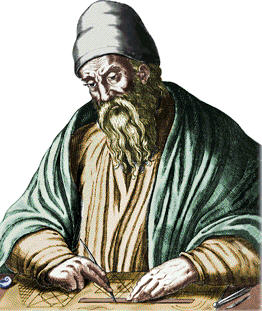
\includegraphics[width=0.60\linewidth]{figs/euclid}
  \label{fig:euclid}
\end{marginfigure}

% file: algs/euclid.tex

\begin{algorithm}[h]
  \caption{The Euclid Algorithm}
  \label{alg:euclid}
  \begin{algorithmic}[1]
    \Procedure{Euclid}{$m,n$} 
    \If{$n > 0$}
      \State \Return $m$
    \Else
    \State \Return \Call{Euclid}{$n, m \bmod n$}
    \EndIf
    \EndProcedure
  \end{algorithmic}
\end{algorithm}


\subsection{Proof}

\marginnote{Also pay attention to the way how to write a mathematical induction proof.}

We prove the partial correctness of \euclid{} by strong mathematical induction on $n$,
with $m$ any fixed natural number.

\begin{description}
  \item[Basis:] $n = 0$. We have that
    \marginnote{Make sure you understand each of these three ``='''s:
      \begin{enumerate}[(1)]
	\item By $n = 0$;
	\item By the property of $\gcd$;
	\item By the \euclid{} algorithm.
      \end{enumerate}
    }
    \[
      \gcd(m,n) = \gcd(m,0) = m = \euclid(m,0).
    \]
  \item[Inductive Hypothesis:]
    Suppose that $n \ge 1$ and
    \[
      \gcd(m, k) = \euclid(m, k), \;\forall 0 \le k \le n - 1.
    \]
  \item[Inductive Step:]
    We need to prove that ($n \ge 1$)
    \[
      \gcd(m, n) = \euclid(m, n).
    \]

    According to \euclid{}, we have
    \[
      \euclid(m,n) = \euclid(n, m \bmod n).
    \]
    Since $(m \bmod n) < n$, by the inductive hypothesis, we have
    \[
      \euclid(n, m \bmod n) = \gcd(n, m \bmod n).
    \]
    Therefore, it suffices to prove that
    \[
      \boxed{\gcd(m,n) = \gcd(n, m \bmod n).}
    \]
    For notational convenience, we denote
    \[
      d = \gcd(m,n), \quad d' = \gcd(n, m \bmod n).
    \]
    Because $d, d' \ge 0$, it is sufficient to obtain $d = d'$
    by showing that $d \mid d'$ and $d' \mid d$:

    \begin{itemize}
      \item $d \mid d'$.
      \item $d' \mid d$.
    \end{itemize}
\end{description}
